% !TeX spellcheck = en_US
\documentclass[12pt, a4paper]{article}
\usepackage{comment}
\usepackage{ragged2e}
\usepackage{amsmath}
\usepackage{xcolor}
\usepackage{multirow}
\usepackage{caption}
\usepackage{tikz}
\usepackage{booktabs}
\usepackage{tabu}
\usepackage{placeins}
\usepackage{pdflscape}
\usetikzlibrary{arrows}
\usepackage{hyperref}
\usepackage{multirow}
\usepackage{subcaption}
 \usepackage{pdflscape}



\captionsetup{font=footnotesize,labelfont=footnotesize}

\hypersetup{
    colorlinks=true,
    linkcolor=blue,
    filecolor=blue,      
    urlcolor=blue,
    citecolor=blue
}

\usepackage{natbib}
\usepackage[title]{appendix}

\tikzstyle{startstop} = [rectangle, rounded corners, minimum width=2cm, minimum height=0.75cm,text centered, draw=black, fill=red!30]

\tikzstyle{startstop1} = [rectangle, rounded corners, minimum width=2cm, minimum height=0.75cm,text centered, draw=black, fill=blue!30]

\tikzstyle{startstop2} = [rectangle, rounded corners, minimum width=2cm, minimum height=0.75cm,text centered, draw=black, fill=yellow!30]

\tikzstyle{startstop3} = [rectangle , rounded corners, minimum width=0.5cm, minimum height=0.75cm,text centered,draw=black]


\tikzstyle{io} = [trapezium, trapezium left angle=70, trapezium right angle=110, minimum width=2cm, minimum height=0.75cm, text centered, draw=black, fill=blue!30]



\tikzstyle{process} = [rectangle, minimum width=2cm, minimum height=1cm, text centered, draw=black, fill=green!30]

\tikzstyle{decision} = [diamond, minimum width=0.75cm, minimum height=0.75cm, text centered, draw=black, fill=green!30]

\tikzstyle{arrow} = [thick,->,>=stealth]



\def\sym#1{\ifmmode^{#1}\else\(^{#1}\)\fi}


\renewcommand{\today}{\ifcase \month \or January\or February\or March\or %
April\or May \or June\or July\or August\or September\or October\or November\or %
December\fi, \number \year} 

\title{{How are stocks connected?\\
\small The evidence from emerging market}}
\author{{S.M. Aghajanzadeh\sym{*} \qquad M. Heidari\sym{*} \qquad M. Mohseni\sym{*} }\\
{\sym{*} \footnotesize  Tehran Institute for Advanced Studies, Khatam University, Tehran, Iran}
}

\def\boxit#1{%
  \smash{\color{red}\fboxrule=1pt\relax\fboxsep=2pt\relax%
  \llap{\rlap{\fbox{\vphantom{0}\makebox[#1]{}}}~}}\ignorespaces
}


\usepackage{lipsum}

\linespread{1.2}




\begin{document}
\maketitle


\begin{abstract}

\end{abstract}





\section{Introduction}


\section{Data and Methodology}



\subsection{Data and Sample}


	 \begin{table}[htbp]
        \centering
        \caption{ This table reports summary statistics of ownership features for all the listed firms. At this table by group, we mean business groups.}
        \label{t2-1}
        \resizebox{1\textwidth}{!}
        {
          \begin{tabular}{lccccccc}
          \hline\hline
          Year  & \multicolumn{1}{c}{2015} & \multicolumn{1}{c}{2016} & \multicolumn{1}{c}{2017} & \multicolumn{1}{c}{2018} & \multicolumn{1}{c}{2019} & \multicolumn{1}{c}{2020} & Meann \\\hline
     No. of Firms & 355   & 383   & 520   & 551   & 579   & 602   & 498 \\
     No. of Blockholders & 724   & 887   & 1274  & 1383  & 1409  & 1390  & 1178 \\
     No. of Groups & 41    & 42    & 46    & 45    & 40    & 40    & 42 \\
     No. of Firms not in Groups & 113   & 128   & 207   & 224   & 247   & 270   & 198 \\
     No. of Firms in Groups & 242   & 265   & 332   & 339   & 332   & 332   & 307 \\
     Mean Number of Members & 6     & 6     & 7     & 8     & 8     & 8     & 7 \\
%     Max. Number of Members & 24    & 25    & 27    & 28    & 28    & 28    & 27 \\
     Med. of Number of Members & 4     & 4     & 6     & 5     & 6     & 6     & 5 \\
     Mean Of each Blockholder's ownership & 21.30 & 22.00 & 20.80 & 20.50 & 21.90 & 23.00 & 21.58 \\
     Med. of Owners' Percent & 7.94  & 7.55  & 6.95  & 6.34  & 8.31  & 9     & 8 \\
     Mean Number of Blockholders & 5     & 5     & 5     & 5     & 5     & 4     & 5 \\
     Med. Number of Owners & 4     & 4     & 4     & 4     & 4     & 3     & 4 \\
%     Max. Number of Owners & 21    & 22    & 28    & 27    & 25    & 24.00 & 25 \\
     Mean Block. Ownership & 71.6  & 71.2  & 68    & 67.7  & 65.4  & 62.00 & 67.65 \\
     Med. Block. Ownership & 79.9  & 80.1  & 77    & 77.1  & 72.9  & 69.70 & 76.12 \\
%     Max. Block. Ownership & 100   & 100   & 100   & 100   & 100   & 100   & 100 \\
          \hline\hline 
%                  \multicolumn{8}{l}{\footnotesize \textit{}}}\\
    
          \end{tabular}
         
         }
      \end{table}


\subsection{Pair composition} 
 \begin{table}
  \centering
  \caption{ This table reports summary statistics of ownership features for total pairs. At this table by group, we mean business groups.}
  \label{t2-2}
    \resizebox{1\textwidth}{!}
          {
 \begin{tabular}{lrrrrrr}
\toprule
Year &   2014 &   2015 &   2016 &   2017 &   2018 &   2019 \\
\midrule
No. of Pairs                       &  18368 &  19285 &  22817 &  37204 &  44722 &  60631 \\
No. of Pairs not in Groups         &   9555 &   9927 &  11831 &  23630 &  27425 &  38474 \\
No. of Pairs not in the same Group &   7564 &   8194 &   9604 &  11748 &  14776 &  19351 \\
No. of Pairs in the same Group     &    893 &    885 &   1038 &   1174 &   1511 &   1698 \\
Ave. Number of Common owner        &      1 &      1 &      1 &      1 &      1 &      1 \\
\bottomrule
\end{tabular}

   }
    \end{table}

\begin{figure}[htbp]
	\centering
	\caption{ Three categories for pairs base on being in business groups}
	\label{g2-1}
	
	\normalcolor
	\begin{subfigure}[t]{0.9\linewidth}
		
		\resizebox{0.49\textwidth}{!}{
			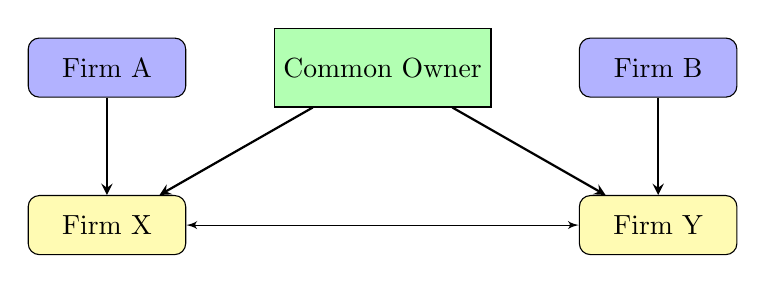
\begin{tikzpicture}[node distance=2cm]
				
				
				
				\node (CH) [process,yshift = -2cm ,xshift=3.5cm] {Common Owner};
				
				\node (end) [startstop1,left of = CH ,xshift=-1.5cm ] {$ \text{Firm A} $};
				
				\node (end2) [startstop1,right of = CH ,yshift=0cm,xshift=1.5cm] {$ \text{Firm B} $};
				
				\node (sur) [startstop2 ,below of = end ,yshift=0cm,xshift=0cm] {$ \text{Firm X} $};
				
				\node (sur2) [startstop2,below of = end2 ,yshift=0cm,xshift=0cm] {$ \text{Firm Y} $};
				
				
				\draw [arrow] (end) --(sur);
				\draw [arrow] (end2) -- (sur2);
				
				
				\draw [arrow] (CH) -- (sur);
				\draw [arrow] (CH) -- (sur2);
				
				\draw [latex'-latex'] (sur) to [bend right =0]  node[sloped, anchor=center, below] {} (sur2);
				
				
			\end{tikzpicture}
		}   
		\hfill
		\resizebox{0.49\textwidth}{!}{
			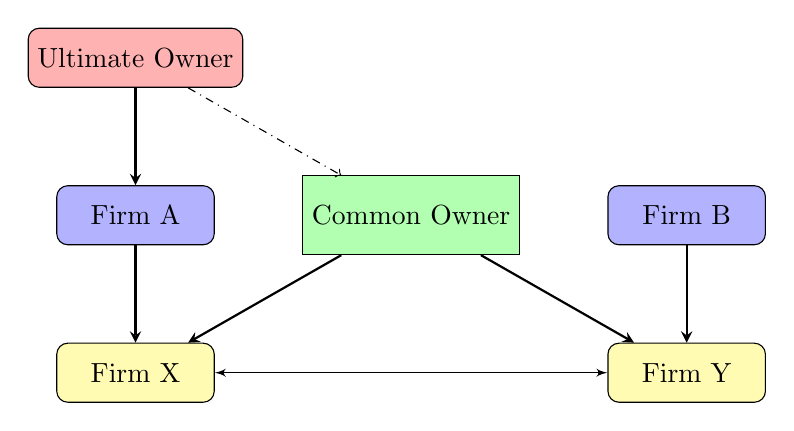
\begin{tikzpicture}[node distance=2cm]
				
				
				\node (start) [startstop] { $ \text{Ultimate Owner} $};
				
				
				\node (CH) [process, below of = start,xshift=3.5cm] {Common Owner};
				
				\node (end) [startstop1,below of = start ] {$ \text{Firm A} $};
				
				\node (end2) [startstop1,right of = CH ,yshift=0cm,xshift=1.5cm] {$ \text{Firm B} $};
				
				\node (sur) [startstop2 ,below of = end ,yshift=0cm,xshift=0cm] {$ \text{Firm X} $};
				
				\node (sur2) [startstop2,below of = end2 ,yshift=0cm,xshift=0cm] {$ \text{Firm Y} $};
				
				
				
				\draw [arrow] (start) --(end);
				
				\draw [arrow] (end) --(sur);
				\draw [arrow] (end2) -- (sur2);
				
				\draw [dash dot,->] (start) -- (CH);
				
				\draw [arrow] (CH) -- (sur);
				\draw [arrow] (CH) -- (sur2);
				
				\draw [latex'-latex'] (sur) to [bend right =0]  node[sloped, anchor=center, below] {} (sur2);
				
				
			\end{tikzpicture}
		}
		\caption{ Pair not in the business group}
	\end{subfigure}
	\bigskip
	\begin{subfigure}[t]{.45\linewidth}
		\centering
		\tiny
		\resizebox{1\textwidth}{!}{
			
			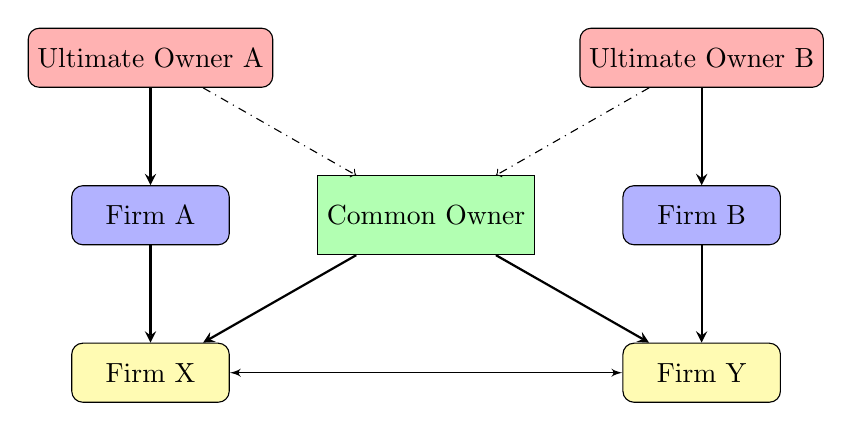
\begin{tikzpicture}[node distance=2cm]
				
				
				\node (start) [startstop] { $ \text{Ultimate Owner A} $};
				\node (start2) [startstop,right of = start,xshift=5cm] {$ \text{Ultimate Owner B} $};
				
				
				\node (CH) [process, below of = start2,xshift=-3.5cm] {Common Owner};
				
				\node (end) [startstop1,below of = start ] {$ \text{Firm A} $};
				
				\node (end2) [startstop1,below of = start2 ,yshift=0cm,xshift=0cm] {$ \text{Firm B} $};
				
				\node (sur) [startstop2 ,below of = end ,yshift=0cm,xshift=0cm] {$ \text{Firm X} $};
				
				\node (sur2) [startstop2,below of = end2 ,yshift=0cm,xshift=0cm] {$ \text{Firm Y} $};
				
				
				
				\draw [arrow] (start) --(end);
				\draw [arrow] (start2) -- (end2);
				
				\draw [arrow] (end) --(sur);
				\draw [arrow] (end2) -- (sur2);
				
				\draw [dash dot,->] (start) -- (CH);
				\draw [dash dot,->] (start2) -- (CH);
				
				\draw [arrow] (CH) -- (sur);
				\draw [arrow] (CH) -- (sur2);
				
				\draw [latex'-latex'] (sur) to [bend right =0]  node[sloped, anchor=center, below] {} (sur2);
				
				
			\end{tikzpicture}
		}   
		\caption{ Pair in two distinct business group}
	\end{subfigure}
	\begin{subfigure}[t]{.45\linewidth}
		\centering
		\tiny
		\resizebox{1\textwidth}{!}{
			
			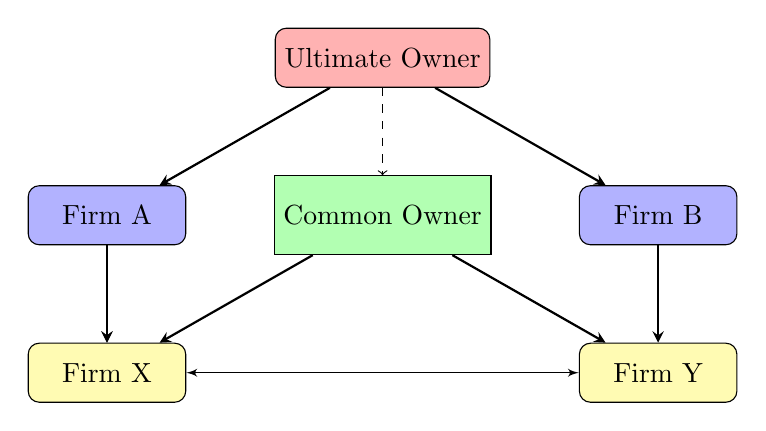
\begin{tikzpicture}[node distance=2cm]
				
				
				\node (start) [startstop] {Ultimate Owner};
				
				
				
				\node (end) [startstop1,below of = start , yshift=0cm , xshift=-3.5cm ] {$ \text{Firm A} $};
				\node (end2) [startstop1,below of = start , yshift=0cm , xshift=3.5cm ] {$ \text{Firm B} $};
				
				
				
				\node (sur) [startstop2 ,below of = end ,yshift=0cm,xshift=0cm] {$ \text{Firm X} $};
				
				
				\node (sur2) [startstop2 ,below of = end2 ,yshift=0cm,xshift=0cm] {$ \text{Firm Y} $};
				
				
				\node (CH) [process, below of = start ,xshift=0] {Common Owner};
				
				
				\draw [arrow] (start) --(end);
				\draw [arrow] (end) --(sur);
				
				\draw [arrow] (start) --(end2);
				
				\draw [arrow] (end) --(sur);
				\draw [arrow] (end2) -- (sur2);
				
				
				\draw [arrow] (CH) -- (sur);
				\draw [arrow] (CH) -- (sur2);
				\draw [dashed ,->] (start) --(CH);
				
				\draw [latex'-latex'] (sur) to [bend right =0]  node[sloped, anchor=center, below] {} (sur2);
				
				
			\end{tikzpicture}
		} 
		
		\caption{ Pair in the same business group}
	\end{subfigure}
	
	
	
\end{figure}  


  \FloatBarrier
  
  
  
\subsection{Stock Return co-movement}
\label{comovement}

 \begin{table}[htbp]
        \centering
        \caption{\footnotesize This table reports distribution of calculated correlation base on different models.}
        \label{tCorr}
        \resizebox{1\textwidth}{!}
        {
        \begin{tabular}{lrrrrr}
\toprule
{} &   mean &    std &    min &  median &    max \\
\midrule
 CAPM + Industry    &  0.019 &  0.127 & -0.925 &   0.015 &  0.902 \\
4 Factor            &  0.032 &  0.136 & -0.877 &   0.023 &  0.837 \\
4 Factor + Industry &  0.015 &  0.125 & -0.903 &   0.012 &  0.755 \\
\bottomrule
\end{tabular}

         }
      \end{table}
      

\FloatBarrier


\subsection{Controls}

\begin{table}[htbp]
\caption{\scriptsize This table reports the number of pairs in the same industry and business group.}
\label{SameGroupIndustry}
               \centering \scriptsize
         {
\begin{tabular}{lll}
\toprule
{} &     Yes &        No \\
\midrule
SameIndustry             &  749265 &  12348105 \\
                         &  (5.7\%) &   (94.3\%) \\
SameGroup                &  302610 &   4480905 \\
                         &  (6.3\%) &   (93.7\%) \\
SameGroup \& SameIndustry &  114840 &  13097370 \\
                         &  (0.9\%) &   (99.1\%) \\
\bottomrule
\end{tabular}

                 }
             \end{table}
 \begin{table}[htbp]
 \caption{\scriptsize This table shows the summary statistics of specified controls in empirical studies.}
 \label{ControlsSummary}
               \centering 
               \scriptsize
                \resizebox{\textwidth}{!}  {
    \begin{tabular}{lrrrrr}
\toprule
{} &  mean &   std &   min &  median &    max \\
\midrule
Size1          &  0.72 &  0.22 &  0.01 &    0.77 &   1.00 \\
Size2          &  0.45 &  0.24 &  0.00 &    0.43 &   0.99 \\
SameSize       & -0.28 &  0.20 & -0.97 &   -0.23 &  -0.00 \\
BM1            &  0.51 &  0.25 &  0.00 &    0.52 &   1.00 \\
BM2            &  0.50 &  0.23 &  0.01 &    0.50 &   1.00 \\
SameBM         & -0.30 &  0.19 & -0.96 &   -0.26 &  -0.00 \\
CrossOwnership &  0.56 &  5.14 &  0.00 &    0.00 &  95.56 \\
\bottomrule
\end{tabular}

                 }
             \end{table}
         
         
 


\FloatBarrier

\subsection{Measurement of common-ownership}

\begin{table}[htbp]
	\centering
	\scriptsize
	\caption{ This table summarizes common ownership measurements in the literature.}
	\label{maasurmentsSummary}
	\resizebox{\textwidth}{!}{
		\begin{tabular}{cllc}
	\hline\hline
	\multicolumn{1}{c}{Group}      & \multicolumn{1}{c}{Paper} & \multicolumn{1}{c}{measurment} & \multicolumn{1}{c}{Flaws} \\
	\hline\hline
	\addlinespace
	\multicolumn{1}{c}{\multirow{5}[2]{*}{Model Based}} &  \cite{harford2011institutional}     &  \scriptsize  $
	\sum_{i\in I^{A,B}}\frac{\alpha_{i,B}}{\alpha_{i,A} + \alpha_{i,B}}     $     & Bi-directional \\
	\addlinespace 
	&  \cite{azar2018anticompetitive}     &  $   \sum_{j} \sum_k s_j s_k \frac{\sum_i \mu_{ij} \nu_{ik}}{\sum_i \mu_{ij} \nu_{ij}}   $     & Industry level \\
	\addlinespace
	&  \cite{gilje2020s}     &    $ \sum_{i = 1}^{I} \alpha_{i,A}g(\beta_{i,A})\alpha_{i,B}    $   & Bi-directional  \\
	\midrule
	\addlinespace 
	\multicolumn{1}{c}{\multirow{7}[5]{*}{Ad hoc}} & \cite{he2017product};      &  \multirow{2}{*}{$ \sum_{i\in I^{A,B}} 1 $}     & invariant to the level   \\
	& \cite{he2019internalizing} & & of ‌common ownership \\
	\addlinespace
	&  \cite{newham2018common}     &   $ \sum_{i\in I^{A,B}} min\{\alpha_{i,A},\alpha_{i,B}\} $    & ? \\
	\addlinespace
	& \multirow{2}{*}{   \cite{AntonPolk} }  &  \multirow{2}{*}{ $ \sum_{i\in I^{A,B}} \alpha_{i,A}\frac{\bar{\nu}_A}{\bar{\nu}_A +\bar{\nu}_B } + \alpha_{i,B}\frac{\bar{\nu}_B}{\bar{\nu}_A +\bar{\nu}_B }  $ }   &  Invariant to the  \\
	& & & decomposition of ownership \\
	\addlinespace
	& \cite{freeman2019effects}; & \multirow{2}{*}{ $ \sum_{i\in I^{A,B}} \alpha_{i,A} \times \sum_{i\in I^{A,B}} \alpha_{i,B} $ }&?\\
	&  \cite{hansen1996externalities} & & ?\\
	\hline\hline
\end{tabular}
	}
\end{table}



\subsubsection{Modified Anton's measure}


				\begin{figure}[htbp]
				\centering
				\caption{ Numeric example 1} 
				\label{gExample1}
				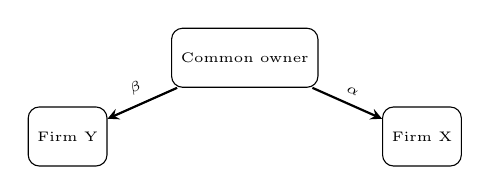
\begin{tikzpicture}[node distance=1cm]
					
					\node (Firm) [startstop3] {\tiny Firm X};
					\node (Firm2) [startstop3,right of = Firm  , xshift=-5.5cm ] {\tiny Firm Y};
					\node (Owner) [startstop3,right of = Firm , yshift=1cm , xshift=-3.25cm ] {\tiny Common owner };
					
					
					\draw[arrow] (Owner) -- node[sloped, anchor=center, above] {\tiny $ \alpha $} (Firm) ;
					
					\draw[arrow] (Owner) -- node[sloped, anchor=center, above] {\tiny $ \beta $} (Firm2) ;
					%
					%\node() at (3,0)
					%    {$ \alpha + \beta = 100 $}; 
				\end{tikzpicture}
			\end{figure}\bigskip

\begin{figure}[htbp]
	\caption{ Comparison of three measure for common ownership}
	\label{example1Results}
	\includegraphics[width=0.47\linewidth]{1.png}
	\includegraphics[width=0.47\linewidth]{2.png}
\end{figure}


			\begin{figure}[htbp]  \centering
				\caption{ Numeric example 2}
				\label{gExample2}
				\centering
				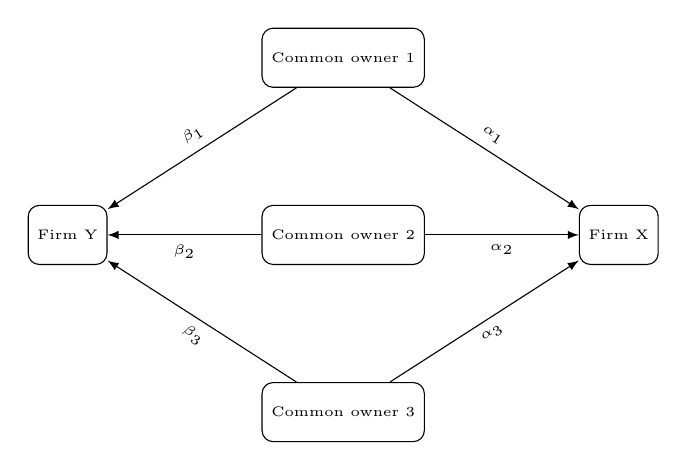
\begin{tikzpicture}[node distance=1cm]
					
					
					\node (Firm) [startstop3] {\tiny Firm X};
					\node (Firm2) [startstop3,right of = Firm , yshift=0cm , xshift=-8cm ] {\tiny Firm Y};
					
					\node (Owner) [startstop3,above of = Firm , yshift=1.25cm , xshift=-3.5cm ] {\tiny Common owner 1 };
					
					
					\node (Owner2) [startstop3,right of = Firm , yshift= 0 , xshift=-4.5cm ] {\tiny Common owner 2 };
					
					\node (Owner3) [startstop3,below of = Firm , yshift=-1.25cm , xshift=-3.5cm ] {\tiny Common owner 3 };
					
					
					
					
					
					\draw [-latex] (Owner) to [bend right =0]  node[sloped, anchor=center, above] {\tiny $ \beta_1 $} (Firm2);
					
					\draw [-latex] (Owner) to [bend left =0]  node[sloped, anchor=center, above] {\tiny $ \alpha_1 $} (Firm);
					
					
					
					\draw [-latex] (Owner2) to [bend right =0]  node[sloped, anchor=center, below] {\tiny $ \beta_2 $} (Firm2);
					
					\draw [-latex] (Owner2) to [bend left =0]  node[sloped, anchor=center, below] {\tiny $ \alpha_2 $} (Firm);
					
					
					
					\draw [-latex] (Owner3) to [bend left =0]  node[sloped, anchor=center, below] {\tiny$ \beta_3 $} (Firm2);
					
					\draw [-latex] (Owner3) to [bend right =0]  node[sloped, anchor=center, below] {\tiny $ \alpha_3 $} (Firm);
					
					
					
				\end{tikzpicture}
			\end{figure}
			\begin{table}[htbp]
				\centering
				\caption{ text}
				\label{Example2}
				\resizebox{1\textwidth}{!}
				{
					    \begin{tabular}{cccccccc}
    \hline\hline
        Ownership  & Type I & Type II & Type III & Type IV & Type V & Type VI & Type VII \\
          \hline
    $ \alpha_1 $    & 1/3 &20      &  10   & 20    & 10    & 5     & 1  \\
    $ \beta_1 $    & 1/3  & 10    & 10   & 20    & 10    & 5     & 1  \\
    $ \alpha_2 $    & 1/3  & 10    & 80    & 20    & 10    & 5     & 1 \\
    $ \beta_2 $    & 1/3  & 20    & 80    & 20    & 10    & 5     & 1  \\
    $ \alpha_3 $    & 1/3  & 70    & 10    & 20    & 10    & 5     & 1 \\
    $ \beta_3 $    & 1/3  & 70    & 10   & 20    & 10    & 5     & 1  \\
    \hline
    SQRT  & 3     &  2.56  & 2.33 & 1.8   & 0.9   & 0.45  & 0.09 \\
    SUM   & 1     & 1     & 1     & 0.6   & 0.3   & 0.15  & 0.03 \\
    Quadratic & 3     & 1.85  & 1.52  & 8.33  & 33.33 & 133.33 & 3333.33 \\
 
    \hline\hline
    \end{tabular}%
				}
			\end{table}
			\begin{figure}[htbp]
				\centering
				\caption{ SQRT measure for fixed aggregate ownership on different relative market cap ratios}
				\label{sqrtMarket}
				\includegraphics[width=0.85\linewidth]{3.png}
			\end{figure}
			\begin{figure}[htbp]
				\centering
				\caption{ Sum measure for fixed aggregate ownership on different relative market cap ratios}
				\label{sumMarket}
				\includegraphics[width=0.85\linewidth]{4.png}
			\end{figure}
			\begin{table}[htbp]
						\centering
						\caption{text }
						\label{marketcap}
						\resizebox{!}{!}
						{
							          \scriptsize
    \begin{tabular}{ccccccc}
    \hline\hline
  & \multicolumn{6}{c}{\tiny($ \alpha_1 $,$ \beta_1 $),($ \alpha_2 $,$ \beta_2 $) }\\ \cmidrule(lr){2-7}
               & \multicolumn{2}{c}{\tiny(10,40),(10,40)} & \multicolumn{2}{c}{\tiny(15,35),(15,35)} & \multicolumn{2}{c}{\tiny(20,30),(20,30)} \\ \cmidrule(lr){2-3}\cmidrule(lr){4-5}\cmidrule(lr){6-7}
    \tiny $ \frac{\text{MarketCap}_x}{\text{MarketCap}_y} $     &\tiny SQRT  & \tiny SUM   &\tiny SQRT  &\tiny SUM   &\tiny SQRT  &\tiny SUM \\ 
     \hline\addlinespace

         1     & 0.90  & 0.50  & 0.96  & 0.50  & 0.99  & 0.50 \\
         2     & 0.80  & 0.40  & 0.89  & 0.43  & 0.96  & 0.47 \\
         3     & 0.75  & 0.35  & 0.85  & 0.40  & 0.94  & 0.45 \\
         4     & 0.71  & 0.32  & 0.83  & 0.38  & 0.92  & 0.44 \\
         5     & 0.69  & 0.30  & 0.81  & 0.37  & 0.91  & 0.43 \\
         6     & 0.67  & 0.29  & 0.80  & 0.36  & 0.91  & 0.43 \\
         7     & 0.65  & 0.28  & 0.79  & 0.35  & 0.90  & 0.43 \\
         8     & 0.64  & 0.27  & 0.78  & 0.34  & 0.90  & 0.42 \\
         9     & 0.63  & 0.26  & 0.77  & 0.34  & 0.89  & 0.42 \\
         10    & 0.62  & 0.25  & 0.76  & 0.34  & 0.89  & 0.42 \\
     
    \hline\hline
    \end{tabular}
						}
				\end{table}
		
		








\begin{table}[htbp]
	\centering
	\caption{ text}
	\label{measureResults}
	\resizebox{1\textwidth}{!}
	{
		\begin{tabular}{lllllllllll}
\toprule
 & \multicolumn{5}{c}{MFCAP} & \multicolumn{5}{c}{FCAP} \\
\cmidrule(lr){2-6}  \cmidrule(lr){7-11} 
 &       mean &    std &    min & median &    max &         mean &    std &    min & median &    max \\
\midrule
All               &      0.158 &  0.234 &  0.002 &  0.079 &  12.65 &        0.144 &  0.166 &  0.002 &  0.077 &    1.0 \\
Same Group        &      0.474 &  0.478 &  0.005 &  0.367 &  6.174 &        0.346 &  0.265 &  0.004 &  0.321 &    1.0 \\
Not Same Group    &      0.147 &  0.212 &  0.002 &  0.077 &  12.65 &        0.137 &  0.157 &  0.002 &  0.074 &    1.0 \\
Same Industry     &      0.274 &  0.383 &  0.003 &  0.126 &  6.262 &        0.207 &  0.215 &  0.003 &   0.12 &  0.999 \\
Not Same Industry &       0.15 &  0.217 &  0.002 &  0.077 &  12.65 &         0.14 &  0.161 &  0.002 &  0.074 &    1.0 \\
\bottomrule
\end{tabular}

	}
\end{table}










\FloatBarrier



\subsection{Overview of Business Groups in Tehran Stock Exchange} \label{BGDef}


		\begin{figure}[htbp]
			\caption{}
			\label{sameIndustryinBG}
			\centering
			\includegraphics[width=0.48\linewidth]{Output/sameIndustryinBG.eps}
			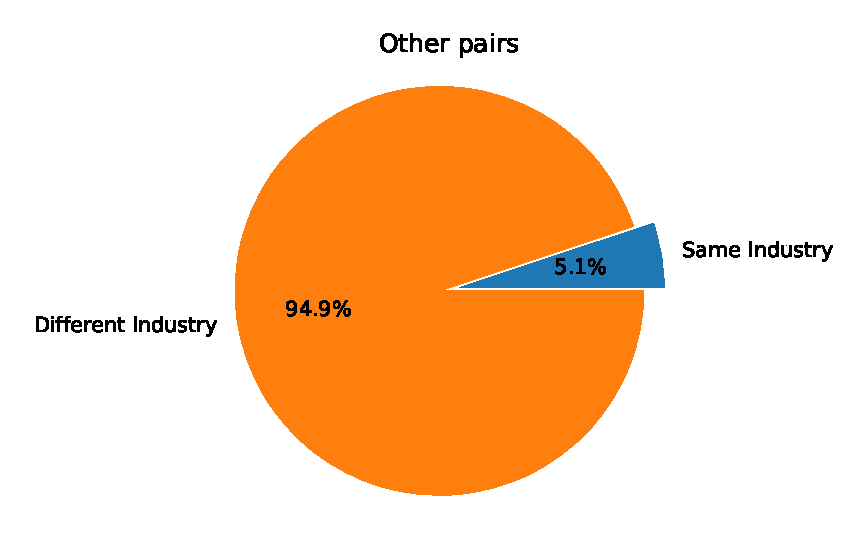
\includegraphics[width=0.48\linewidth]{Output/sameIndustryNoinBG.eps}
		\end{figure}

	\begin{figure}[htbp]
		\caption{}
		\label{BGSummary}
		\centering
		\includegraphics[width=0.85\linewidth]{Output/BGSummary.eps}
	\end{figure}



\FloatBarrier




\section{Results}



\subsection{Forecasting Co-movement}
\label{Forecasting Co-movement}


	 \begin{figure}[htbp]
		\centering  
		\centering
		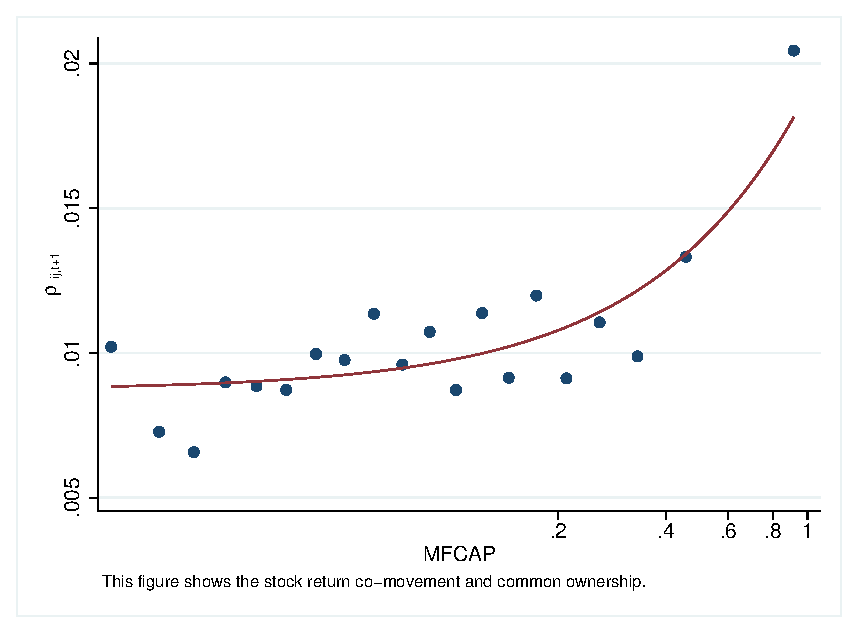
\includegraphics[width=0.7\linewidth]{"Output/mcorr50.eps"} 
		\caption{Future monthly correlation for different level of common ownership at this period }
		\label{mcorr50}
	\end{figure}
	

 \begin{landscape}

	{\begin{table}[htbp]
%	\centering
	\caption{Connected Co-movement}
	\label{mresult2}
%	\resizebox{1\textwidth}{!}{
		{
\def\sym#1{\ifmmode^{#1}\else\(^{#1}\)\fi}
\begin{tabular}{l*{9}{c}}
\hline\hline
                &\multicolumn{9}{c}{Dependent Variable: Future Monthly Correlation of 4F+Industry Residuals}                                                                               \\\cmidrule(lr){2-10}
                &\multicolumn{1}{c}{(1)}         &\multicolumn{1}{c}{(2)}         &\multicolumn{1}{c}{(3)}         &\multicolumn{1}{c}{(4)}         &\multicolumn{1}{c}{(5)}         &\multicolumn{1}{c}{(6)}         &\multicolumn{1}{c}{(7)}         &\multicolumn{1}{c}{(8)}         &\multicolumn{1}{c}{(9)}         \\
\hline
Same Group      &   0.0166\sym{***}&   0.0153\sym{***}&                  &                  &   0.0147\sym{***}&                  &                  &  0.00624\sym{***}&  0.00549\sym{**} \\
                &   (8.54)         &   (7.90)         &                  &                  &   (6.97)         &                  &                  &   (2.81)         &   (2.27)         \\
[1em]
$ \text{FCA*} $ &                  &                  &  0.00150\sym{***}&  0.00112\sym{**} & 0.000736         &  0.00944\sym{***}& 0.000397         & 0.000377         &-0.0000113         \\
                &                  &                  &   (2.90)         &   (2.11)         &   (1.33)         &   (7.24)         &   (0.68)         &   (0.65)         &  (-0.02)         \\
[1em]
 $ (\text{FCA}^*) \times {\text{SameGroup} }  $ &                  &                  &                  &                  &                  &                  &                  &  0.00992\sym{***}&   0.0107\sym{***}\\
                &                  &                  &                  &                  &                  &                  &                  &   (6.49)         &   (6.97)         \\
\hline
Observations    &  1665996         &  1665996         &  1665996         &  1665996         &  1665996         &    58337         &  1607659         &  1665996         &  1665996         \\
Sub-sample      &      All         &      All         &      All         &      All         &      All         &SameGroup         &   Others         &      All         &      All         \\
Group Effect    &       No         &       No         &       No         &       No         &       No         &       No         &       No         &       No         &      Yes         \\
Controls        &       No         &      Yes         &       No         &      Yes         &      Yes         &      Yes         &      Yes         &      Yes         &      Yes         \\
$ R^2 $         & 0.000180         & 0.000637         & 0.000170         & 0.000652         & 0.000804         &   0.0112         & 0.000577         & 0.000898         &  0.00575         \\
\hline\hline
\multicolumn{10}{l}{\footnotesize \textit{t} statistics in parentheses}\\
\multicolumn{10}{l}{\footnotesize \sym{*} \(p<0.10\), \sym{**} \(p<0.05\), \sym{***} \(p<0.01\)}\\
\end{tabular}
}

%	}
\end{table}}
 \end{landscape}
\FloatBarrier



\subsection{High level of common ownership}

	\begin{figure}[htbp]
		\centering  
		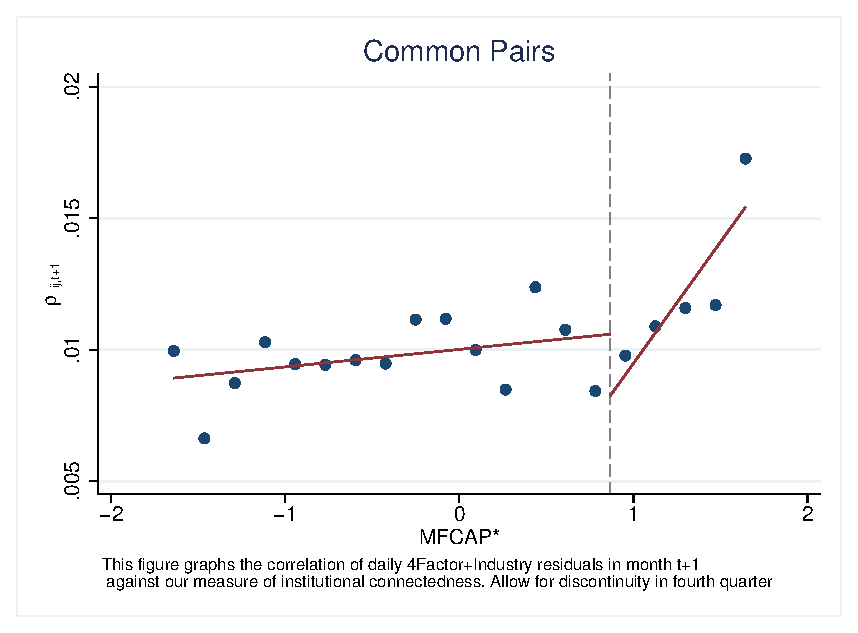
\includegraphics[width=0.6\linewidth]{"Output/Qmcorr5lrd.eps"}
		\caption{text}
		\label{Qmcorr5lrd}
	\end{figure}
	\begin{figure}[htbp]
		\centering  
		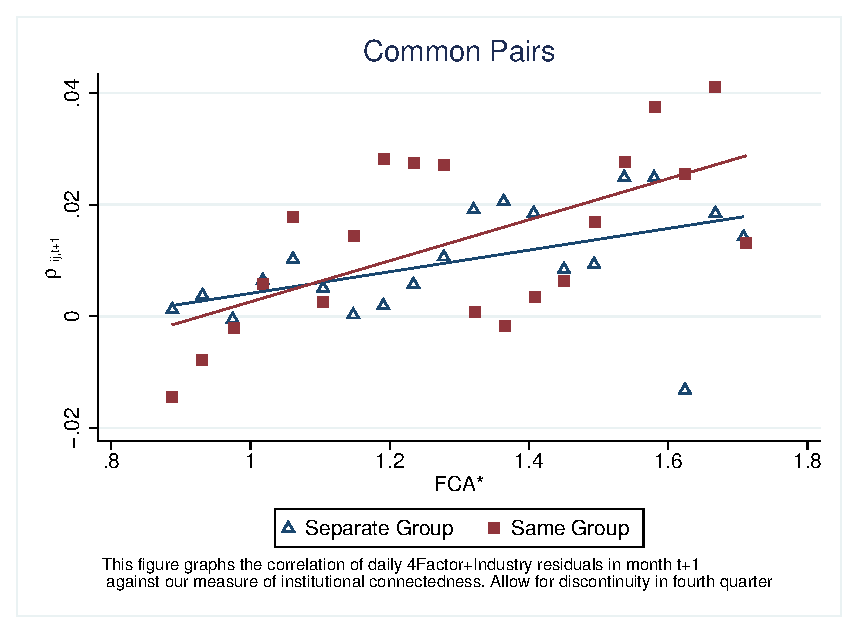
\includegraphics[width=0.45\linewidth]{"Output/Qmcorr5lrdbgsubsample.eps"}
		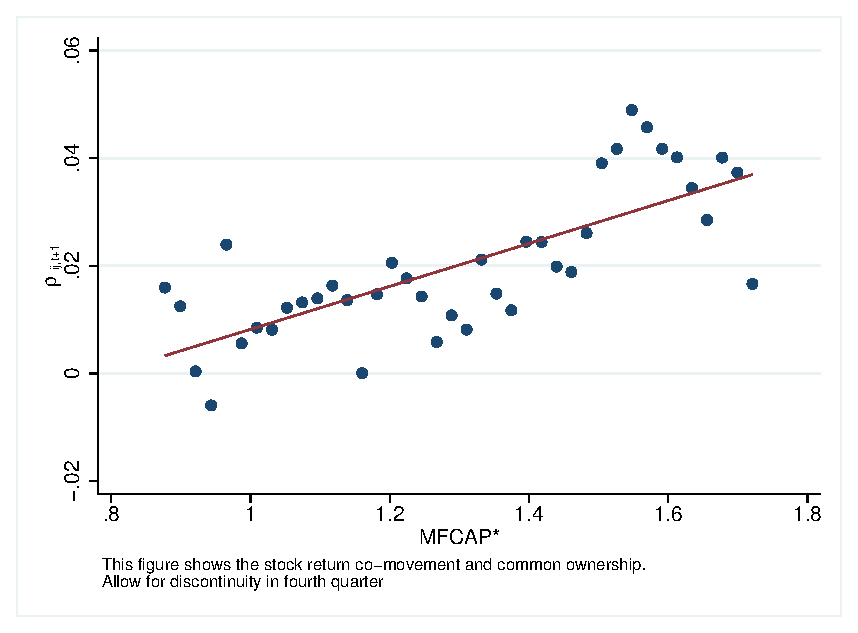
\includegraphics[width=0.45\linewidth]{"Output/Qmcorr5subsample.eps"}
		\caption{text}
		\label{Qmcorr5subsample}
	\end{figure}
 \begin{table}[htbp]
	 	\centering
	 	\caption{\scriptsize Estimation results for high level of common ownership}
	 	\label{QTimemresult2subsample}
	 	\resizebox{0.75\textwidth}{!}{
	 		{
\def\sym#1{\ifmmode^{#1}\else\(^{#1}\)\fi}
\begin{tabular}{l*{4}{c}}
\hline\hline
                &\multicolumn{4}{c}{Dependent Variable: Standardized Future Pairs's co-movement}\\\cmidrule(lr){2-5}
                &\multicolumn{1}{c}{(1)}         &\multicolumn{1}{c}{(2)}         &\multicolumn{1}{c}{(3)}         &\multicolumn{1}{c}{(4)}         \\
\hline
Same Group      &   0.0740\sym{***}&                  &   -0.112\sym{*}  &   -0.102\sym{*}  \\
                &   (8.36)         &                  &  (-2.58)         &  (-2.30)         \\
[1em]
$ \text{MFCAP*} $&                  &   0.0115         &  -0.0214         &  -0.0212\sym{*}  \\
                &                  &   (1.07)         &  (-1.93)         &  (-2.01)         \\
[1em]
 $ (\text{MFCAP}^*) \times {\text{SameGroup} }  $ &                  &                  &    0.131\sym{***}&    0.124\sym{***}\\
                &                  &                  &   (4.30)         &   (3.96)         \\
\hline
Controls        &      Yes         &      Yes         &      Yes         &      Yes         \\
Business Group FE&       No         &       No         &       No         &      Yes         \\
Observations    &   360050         &   360050         &   360050         &   360050         \\
\hline\hline
\multicolumn{5}{l}{\footnotesize \textit{t} statistics in parentheses}\\
\multicolumn{5}{l}{\footnotesize \sym{*} \(p<0.05\), \sym{**} \(p<0.01\), \sym{***} \(p<0.001\)}\\
\end{tabular}
}

	 	}
	 \end{table}

	
			\begin{figure}[htbp]
				\centering  
				\includegraphics[width=0.75\linewidth]{"Output/QarterSummary.eps"}
				\caption{Pairs' characteristics for the pairs with high level of common ownership}
				\label{QarterSummary}
			\end{figure}


\FloatBarrier

\subsection{All Pairs}

\begin{landscape}

	\begin{table}[htbp]
		%	\centering
		\caption{Non-connected Co-movement}
		\label{AllPairs}
		\resizebox{1.7\textwidth}{!}{
			{
\def\sym#1{\ifmmode^{#1}\else\(^{#1}\)\fi}
\begin{tabular}{l*{7}{c}}
\hline\hline
                &\multicolumn{7}{c}{Dependent Variable: Future Pairs' co-movement}                                                                   \\\cmidrule(lr){2-8}
                &\multicolumn{1}{c}{(1)}         &\multicolumn{1}{c}{(2)}         &\multicolumn{1}{c}{(3)}         &\multicolumn{1}{c}{(4)}         &\multicolumn{1}{c}{(5)}         &\multicolumn{1}{c}{(6)}         &\multicolumn{1}{c}{(7)}         \\
\hline
SameGroup       &   0.0153\sym{***}&                  &   0.0150\sym{***}&                  &                  &   0.0134\sym{***}&   0.0124\sym{***}\\
                &   (9.38)         &                  &   (9.26)         &                  &                  &   (7.81)         &   (7.10)         \\
[1em]
$ \text{MFCAP*} $&                  & 0.000676\sym{***}& 0.000496\sym{*}  &  0.00212         & 0.000427\sym{*}  & 0.000408\sym{*}  & 0.000116         \\
                &                  &   (3.50)         &   (2.56)         &   (1.79)         &   (2.20)         &   (2.11)         &   (0.67)         \\
[1em]
 $ (\text{MFCAP}^*) \times {\text{SameGroup} }  $ &                  &                  &                  &                  &                  &  0.00247\sym{*}  &  0.00321\sym{**} \\
                &                  &                  &                  &                  &                  &   (2.15)         &   (2.90)         \\
\hline
Observations    &  6018646         &  6018646         &  6018646         &   114526         &  5904120         &  6018646         &  6018646         \\
Sub Sample      &    Total         &    Total         &    Total         &SameGroups         &   Others         &    Total         &    Total         \\
Group Effect    &       No         &       No         &       No         &       No         &       No         &       No         &      Yes         \\
Controls        &      Yes         &      Yes         &      Yes         &      Yes         &      Yes         &      Yes         &      Yes         \\
$ R^2 $         & 0.000445         & 0.000392         & 0.000491         &  0.00699         & 0.000338         & 0.000515         &  0.00330         \\
\hline\hline
\multicolumn{8}{l}{\footnotesize \textit{t} statistics in parentheses}\\
\multicolumn{8}{l}{\footnotesize \sym{*} \(p<0.05\), \sym{**} \(p<0.01\), \sym{***} \(p<0.001\)}\\
\end{tabular}
}

		}
	\end{table}
\end{landscape}


\FloatBarrier




\subsection{Size effect}

	\begin{figure}[htbp]
		\centering  
		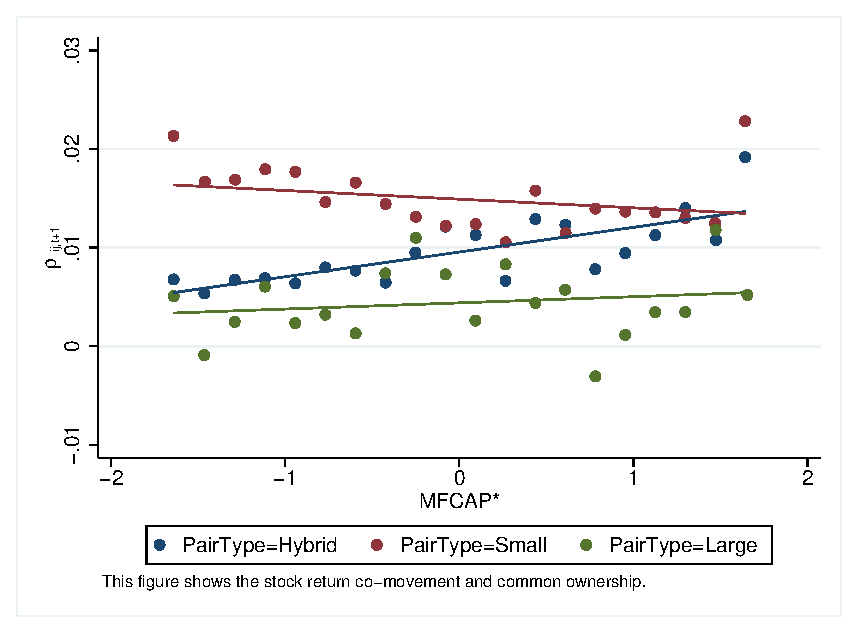
\includegraphics[width=0.7\linewidth]{"Output/mcorrPairType.eps"}
		\caption{text}
		\label{mcorrPairType}
	\end{figure}

		\begin{table}[htbp]
				\centering
				\caption{text}
				\label{Qmresult4}
				\resizebox{1\textwidth}{!}{
					{
\def\sym#1{\ifmmode^{#1}\else\(^{#1}\)\fi}
\begin{tabular}{l*{8}{c}}
\hline\hline
                &\multicolumn{8}{c}{Dependent Variable: Future Monthly Correlation of 4F+Ind. Res.}                                                                     \\\cmidrule(lr){2-9}
                &\multicolumn{1}{c}{(1)}         &\multicolumn{1}{c}{(2)}         &\multicolumn{1}{c}{(3)}         &\multicolumn{1}{c}{(4)}         &\multicolumn{1}{c}{(5)}         &\multicolumn{1}{c}{(6)}         &\multicolumn{1}{c}{(7)}         &\multicolumn{1}{c}{(8)}         \\
\hline
Same Group      &  0.00624\sym{**} &   0.0102\sym{***}& -0.00153         &   0.0117\sym{***}&  0.00661\sym{*}  &   0.0366\sym{***}&   0.0268\sym{***}&  0.00750\sym{***}\\
                &   (2.81)         &   (3.95)         &  (-0.53)         &   (3.76)         &   (2.15)         &  (10.31)         &   (6.57)         &   (3.53)         \\
[1em]
$ \text{FCA*} $ & 0.000377         & 0.000698         &-0.000175         &  0.00199\sym{***}&  0.00177\sym{**} & -0.00151         & -0.00177         &-0.0000771         \\
                &   (0.65)         &   (1.25)         &  (-0.31)         &   (3.56)         &   (3.00)         &  (-1.58)         &  (-1.84)         &  (-0.14)         \\
[1em]
 $ (\text{FCA}^*) \times {\text{SameGroup} }  $ &  0.00992\sym{***}&                  &   0.0134\sym{***}&                  &  0.00599\sym{*}  &                  &   0.0123\sym{***}&   0.0105\sym{***}\\
                &   (6.49)         &                  &   (4.80)         &                  &   (2.34)         &                  &   (4.17)         &   (6.72)         \\
\hline
Observations    &  1665996         &   346170         &   346170         &   693728         &   693728         &   626098         &   626098         &  1665996         \\
Controls        &      Yes         &      Yes         &      Yes         &      Yes         &      Yes         &      Yes         &      Yes         &      Yes         \\
Sub-sample      &All Firms         &Large Firms         &Large Firms         &Hybrid Firms         &Hybrid Firms         &Small Firms         &Small Firms         &All Firms         \\
Pair Size FE    &       No         &       No         &       No         &       No         &       No         &       No         &       No         &      Yes         \\
$ R^2 $         & 0.000898         &  0.00193         &  0.00232         &  0.00135         &  0.00149         &  0.00180         &  0.00198         &  0.00130         \\
\hline\hline
\multicolumn{9}{l}{\footnotesize \textit{t} statistics in parentheses}\\
\multicolumn{9}{l}{\footnotesize \sym{*} \(p<0.05\), \sym{**} \(p<0.01\), \sym{***} \(p<0.001\)}\\
\end{tabular}
}

				}
		\end{table}
		\begin{table}[htbp]
				\centering
				\caption{text}
				\label{Qmresult4AllPairs}
				\resizebox{1\textwidth}{!}{
					{
\def\sym#1{\ifmmode^{#1}\else\(^{#1}\)\fi}
\begin{tabular}{l*{8}{c}}
\hline\hline
                &\multicolumn{8}{c}{Dependent Variable: Future Monthly Correlation of 4F+Ind. Res.}                                                                     \\\cmidrule(lr){2-9}
                &\multicolumn{1}{c}{(1)}         &\multicolumn{1}{c}{(2)}         &\multicolumn{1}{c}{(3)}         &\multicolumn{1}{c}{(4)}         &\multicolumn{1}{c}{(5)}         &\multicolumn{1}{c}{(6)}         &\multicolumn{1}{c}{(7)}         &\multicolumn{1}{c}{(8)}         \\
\hline
SameGroup       &   0.0134\sym{***}&  0.00954\sym{***}&  0.00853\sym{***}&   0.0136\sym{***}&   0.0118\sym{***}&   0.0314\sym{***}&   0.0267\sym{***}&   0.0138\sym{***}\\
                &   (7.81)         &   (4.63)         &   (3.71)         &   (7.35)         &   (6.46)         &  (10.19)         &   (7.93)         &   (8.27)         \\
[1em]
$ \text{FCA*} $ & 0.000408\sym{*}  &-0.0000120         &-0.000115         & 0.000514\sym{*}  & 0.000401         & -0.00143\sym{***}& -0.00154\sym{***}&-0.000390\sym{**} \\
                &   (2.11)         &  (-0.05)         &  (-0.47)         &   (2.09)         &   (1.67)         &  (-3.86)         &  (-3.97)         &  (-2.70)         \\
[1em]
 $ (\text{FCA}^*) \times {\text{SameGroup} }  $ &  0.00247\sym{*}  &                  &  0.00178         &                  &  0.00272         &                  &  0.00545\sym{**} &  0.00313\sym{**} \\
                &   (2.15)         &                  &   (1.30)         &                  &   (1.59)         &                  &   (3.38)         &   (2.80)         \\
\hline
Observations    &  6018646         &  1753614         &  1753614         &  2992221         &  2992221         &  1272811         &  1272811         &  6018646         \\
Controls        &      Yes         &      Yes         &      Yes         &      Yes         &      Yes         &      Yes         &      Yes         &      Yes         \\
Sub-sample      &All Firms         &Large Firms         &Large Firms         &Hybrid Firms         &Hybrid Firms         &Small Firms         &Small Firms         &All Firms         \\
Pair Size FE    &       No         &       No         &       No         &       No         &       No         &       No         &       No         &      Yes         \\
$ R^2 $         & 0.000515         & 0.000796         & 0.000860         & 0.000688         & 0.000735         &  0.00191         &  0.00199         & 0.000829         \\
\hline\hline
\multicolumn{9}{l}{\footnotesize \textit{t} statistics in parentheses}\\
\multicolumn{9}{l}{\footnotesize \sym{*} \(p<0.05\), \sym{**} \(p<0.01\), \sym{***} \(p<0.001\)}\\
\end{tabular}
}

				}
		\end{table}


\FloatBarrier

\subsection{Common Ownership measure}

{\begin{table}[htbp]
		%	\centering
		\caption{Connected Co-movement}
		\label{mresult2Polk}
		\resizebox{1\textwidth}{!}{
		{
\def\sym#1{\ifmmode^{#1}\else\(^{#1}\)\fi}
\begin{tabular}{l*{7}{c}}
\hline\hline
                &\multicolumn{7}{c}{Dependent Variable: Future Monthly Correlation of 4F+Industry Residuals}                                         \\\cmidrule(lr){2-8}
                &\multicolumn{1}{c}{(1)}         &\multicolumn{1}{c}{(2)}         &\multicolumn{1}{c}{(3)}         &\multicolumn{1}{c}{(4)}         &\multicolumn{1}{c}{(5)}         &\multicolumn{1}{c}{(6)}         &\multicolumn{1}{c}{(7)}         \\
\hline
$ \text{FCAP*} $&  0.00349\sym{***}&  0.00275\sym{***}&  0.00129         & 0.000761         & 0.000928         & 0.000671         &  0.00108         \\
                &   (4.69)         &   (4.75)         &   (1.98)         &   (1.09)         &   (1.46)         &   (1.05)         &   (1.70)         \\
[1em]
 $ (\text{FCAP}^*) \times {\text{SameGroup} }  $ &                  &                  &                  &  0.00662\sym{*}  &  0.00670\sym{*}  &  0.00808\sym{**} &  0.00795\sym{**} \\
                &                  &                  &                  &   (2.20)         &   (2.21)         &   (3.12)         &   (3.15)         \\
[1em]
SameGroup       &                  &                  &   0.0154\sym{***}&  0.00919\sym{**} &   0.0110\sym{***}&  0.00871\sym{**} &  0.00753\sym{*}  \\
                &                  &                  &   (6.66)         &   (3.13)         &   (3.74)         &   (2.76)         &   (2.27)         \\
[1em]
 $ {\rho_t} $   &                  &    0.129\sym{***}&    0.129\sym{***}&    0.129\sym{***}&    0.129\sym{***}&    0.129\sym{***}&    0.129\sym{***}\\
                &                  &   (4.94)         &   (4.93)         &   (4.92)         &   (4.92)         &   (4.92)         &   (4.91)         \\
[1em]
SameIndustry    &                  &                  &                  &                  & -0.00480\sym{*}  & -0.00587\sym{**} & -0.00568\sym{**} \\
                &                  &                  &                  &                  &  (-2.16)         &  (-2.82)         &  (-2.67)         \\
[1em]
SameSize        &                  &                  &                  &                  &                  &  0.00892\sym{***}&  0.00894\sym{***}\\
                &                  &                  &                  &                  &                  &   (4.18)         &   (4.01)         \\
[1em]
SameBookToMarket&                  &                  &                  &                  &                  &  0.00137         &  0.00220         \\
                &                  &                  &                  &                  &                  &   (0.61)         &   (0.94)         \\
[1em]
CrossOwnership  &                  &                  &                  &                  &                  &   0.0223\sym{*}  &   0.0215\sym{*}  \\
                &                  &                  &                  &                  &                  &   (2.22)         &   (2.02)         \\
\hline
Observations    &   436735         &   434850         &   434850         &   434850         &   434850         &   434850         &   434850         \\
Group FE        &       No         &       No         &       No         &       No         &       No         &       No         &      Yes         \\
$ R^2 $         & 0.000316         &   0.0355         &   0.0358         &   0.0360         &   0.0362         &   0.0366         &   0.0432         \\
\hline\hline
\multicolumn{8}{l}{\footnotesize \textit{t} statistics in parentheses}\\
\multicolumn{8}{l}{\footnotesize \sym{*} \(p<0.05\), \sym{**} \(p<0.01\), \sym{***} \(p<0.001\)}\\
\end{tabular}
}
}
\end{table}}

\FloatBarrier


\section{Evidence for correlated trading }


 \subsection{Institutional Imbalance}
\begin{table}[htbp]
 			\centering
 			\caption{text}
 			\resizebox{0.75\textwidth}{!}{
 				\begin{tabular}{lrrrrrrrr}
\toprule
{} &  Group \$\textbackslash times\$ Month &   mean &    std &  min &    25\% &    50\% &    75\% &  max \\
Grouped   &                       &        &        &      &        &        &        &      \\
\midrule
Ungrouped &                 20197 &  0.010 &  0.630 & -1.0 & -0.474 &  0.016 &  0.479 &  1.0 \\
Grouped   &                 12021 & -0.041 &  0.581 & -1.0 & -0.462 & -0.009 &  0.341 &  1.0 \\
\bottomrule
\end{tabular}

 			}
 			\label{tab:ImbalanceInsMeanSummary}
 	\end{table}
 \begin{table}[htbp]
 			\centering
 			\caption{text}
 			\resizebox{0.75\textwidth}{!}{
 				\begin{tabular}{lcccccccc}
\toprule
IndImbalance\_value &        &       &      &        &      &       &     \\
             count &   mean &   std &  min &    25\% &  50\% &   75\% & max \\
             20896 & -0.043 & 0.264 & -1.0 & -0.079 & -0.0 & 0.042 & 1.0 \\
\midrule
             12177 & -0.026 & 0.210 & -1.0 & -0.070 &  0.0 & 0.052 & 1.0 \\
\bottomrule
\end{tabular}

 			}
 			\label{tab:ImbalanceIndMeanSummary}
 	\end{table}
 \FloatBarrier
 

 \begin{table}[htbp]
 				\centering
 				\caption{text}
 				\resizebox{0.75\textwidth}{!}{
 					\begin{tabular}{lcccccccc}
\toprule
{} &  Group \$\textbackslash times\$ Month &   mean &    std &    min &    25\% &    50\% &    75\% &    max \\
\midrule
Ungrouped &                    72 &  0.619 &  0.054 &  0.481 &  0.594 &  0.627 &  0.655 &  0.734 \\
Grouped   &                  2062 &  0.497 &  0.247 &  0.000 &  0.334 &  0.495 &  0.636 &  1.414 \\
\bottomrule
\end{tabular}

 				}
 				\label{tab:ImbalanceInsStdSummary}%
 		\end{table}
 	\begin{table}[htbp]
 				\centering
 				\caption{text}
 				\resizebox{0.75\textwidth}{!}{
 					\begin{tabular}{lcccccccc}
\toprule
{} & IndImbalance\_value &        &        &       &        &        &        &        \\
{} &              count &   mean &    std &   min &    25\% &    50\% &    75\% &    max \\
\midrule
Ungrouped &                 72 &  0.259 &  0.060 &  0.12 &  0.225 &  0.273 &  0.302 &  0.354 \\
Grouped   &               2062 &  0.165 &  0.139 &  0.00 &  0.065 &  0.129 &  0.226 &  1.038 \\
\bottomrule
\end{tabular}

 				}
 				\label{tab:ImbalanceIndStdSummary}
 		\end{table}
 		
 	\begin{figure}[htbp]
 		\centering
 		\caption{text}
 		\includegraphics[width=0.85\linewidth]{Output/GroupedInsSTD.eps}
 		\label{fig:GroupedInsSTD}
 	\end{figure}
 	\begin{figure}[htbp]
 		\centering
 		\caption{text}
 		\includegraphics[width=0.85\linewidth]{Output/GroupedIndSTD.eps}
 		\label{fig:GroupedIndSTD}
 	\end{figure}
 \begin{table}[htbp]
		\centering
		\caption{text}
		\label{Imbalance}
		\resizebox{\textwidth}{!}{
			{
\def\sym#1{\ifmmode^{#1}\else\(^{#1}\)\fi}
\begin{tabular}{l*{7}{c}}
\hline\hline
                &\multicolumn{7}{c}{Future Monthly Corr. of 4F+Ind. Residuals}                                                                       \\\cmidrule(lr){2-8}
                &\multicolumn{1}{c}{(1)}         &\multicolumn{1}{c}{(2)}         &\multicolumn{1}{c}{(3)}         &\multicolumn{1}{c}{(4)}         &\multicolumn{1}{c}{(5)}         &\multicolumn{1}{c}{(6)}         &\multicolumn{1}{c}{(7)}         \\
\hline
$ \text{FCA*} $ &  0.00296\sym{***}&  0.00277\sym{***}&  0.00275\sym{***}&                  &  0.00611\sym{**} &  0.00244\sym{**} &  0.00284\sym{**} \\
                &   (3.77)         &   (3.57)         &   (3.55)         &                  &   (3.21)         &   (3.14)         &   (3.40)         \\
[1em]
Same Group      &  0.00978\sym{***}&  0.00981\sym{***}&  0.00858\sym{**} &   0.0110\sym{***}&                  &  0.00861\sym{**} &  0.00826\sym{**} \\
                &   (4.29)         &   (4.35)         &   (3.37)         &   (4.73)         &                  &   (3.38)         &   (3.05)         \\
[1em]
Low Imbalance std&                  & -0.00364\sym{**} & -0.00388\sym{**} & -0.00446\sym{**} & -0.00725\sym{*}  & -0.00393\sym{**} & 0.000437         \\
                &                  &  (-2.81)         &  (-2.83)         &  (-3.24)         &  (-2.47)         &  (-2.87)         &   (0.21)         \\
[1em]
 $ \text{Low Imbalance std} \times {\text{SameGroup} } $ &                  &                  &  0.00301         &  0.00365         &                  & -0.00904         & -0.00990\sym{*}  \\
                &                  &                  &   (0.81)         &   (0.98)         &                  &  (-1.84)         &  (-2.02)         \\
[1em]
 $ \text{Low Imbalance std} \times {\text{SameGroup} } \times \text{FCA}^*  $ &                  &                  &                  &                  &                  &   0.0104\sym{***}&  0.00941\sym{***}\\
                &                  &                  &                  &                  &                  &   (3.87)         &   (3.53)         \\
\hline
Observations    &   388492         &   388492         &   388492         &   388492         &    37114         &   388492         &   388492         \\
Group Effect    &       No         &       No         &       No         &       No         &       No         &       No         &      Yes         \\
Sub-sample      &    Total         &    Total         &    Total         &    Total         &Same Groups         &    Total         &    Total         \\
Controls        &      Yes         &      Yes         &      Yes         &      Yes         &      Yes         &      Yes         &      Yes         \\
$ R^2 $         &  0.00229         &  0.00255         &  0.00274         &  0.00246         &   0.0199         &  0.00290         &  0.00906         \\
\hline\hline
\multicolumn{8}{l}{\footnotesize \textit{t} statistics in parentheses}\\
\multicolumn{8}{l}{\footnotesize \sym{*} \(p<0.05\), \sym{**} \(p<0.01\), \sym{***} \(p<0.001\)}\\
\end{tabular}
}

		}
	\end{table}
\FloatBarrier

 \subsection{Turnover}
\begin{table}[htbp]
				\centering
				\caption{cross-sectional average of the time-series coefficients for daily changes in turnover }
				\resizebox{0.7\textheight}{!}{
					{
\def\sym#1{\ifmmode^{#1}\else\(^{#1}\)\fi}
\begin{tabular}{l*{4}{c}}
\hline\hline
                    &\multicolumn{4}{c}{Dependent Variable: $\Delta \text{TurnOver}_{i} $ }                 \\\cmidrule(lr){2-5}
                    &\multicolumn{1}{c}{(1)}         &\multicolumn{1}{c}{(2)}         &\multicolumn{1}{c}{(3)}         &\multicolumn{1}{c}{(4)}         \\
\hline
 $ \Delta \text{TurnOver}_{\text{Market}} $ &       0.416\sym{***}&       0.326\sym{***}&       0.252\sym{***}&       0.228\sym{***}\\
                    &     (12.25)         &      (5.35)         &      (6.41)         &      (4.24)         \\
[1em]
 $ \Delta \text{TurnOver}_{\text{Industry-i}} $ &       0.142\sym{***}&       0.213\sym{***}&      0.0335         &       0.167\sym{**} \\
                    &      (3.79)         &      (6.29)         &      (1.34)         &      (2.87)         \\
[1em]
 $ \Delta \text{TurnOver}_{\text{Group,-i}} $ &                     &                     &       0.330\sym{***}&       0.218\sym{***}\\
                    &                     &                     &     (12.74)         &      (3.80)         \\
\hline
Control             &          No         &         Yes         &          No         &         Yes         \\
Observations        &      854662         &      851772         &      333789         &      331263         \\
$ R^2 $             &       0.285         &       0.543         &       0.433         &       0.712         \\
\hline\hline
\multicolumn{5}{l}{\footnotesize \textit{t} statistics in parentheses}\\
\multicolumn{5}{l}{\footnotesize \sym{*} \(p<0.05\), \sym{**} \(p<0.01\), \sym{***} \(p<0.001\)}\\
\end{tabular}
}

				} \label{turnover}
		\end{table}
	\begin{table}[htbp]
					\centering
					\caption{cross-sectional variation in $\beta_{Group}$ }
					\resizebox{0.7\textheight}{!}{
						{
\def\sym#1{\ifmmode^{#1}\else\(^{#1}\)\fi}
\begin{tabular}{l*{10}{c}}
\hline\hline
                &\multicolumn{10}{c}{Dependent Variable: $ \beta_{Group} $ }                                                                                                                                  \\\cmidrule(lr){2-11}
                &\multicolumn{1}{c}{(1)}         &\multicolumn{1}{c}{(2)}         &\multicolumn{1}{c}{(3)}         &\multicolumn{1}{c}{(4)}         &\multicolumn{1}{c}{(5)}         &\multicolumn{1}{c}{(6)}         &\multicolumn{1}{c}{(7)}         &\multicolumn{1}{c}{(8)}         &\multicolumn{1}{c}{(9)}         &\multicolumn{1}{c}{(10)}         \\
\hline
Excess          &    0.681\sym{***}&    0.787\sym{***}&                  &                  &                  &                  &                  &                  &                  &                  \\
                &   (5.59)         &   (6.55)         &                  &                  &                  &                  &                  &                  &                  &                  \\
[1em]
ExcessDummy     &                  &                  &   0.0711         &    0.103\sym{*}  &                  &                  &                  &                  &                  &                  \\
                &                  &                  &   (1.15)         &   (1.98)         &                  &                  &                  &                  &                  &                  \\
[1em]
ExcessDiff      &                  &                  &                  &                  &    1.152\sym{***}&    0.889\sym{***}&                  &                  &                  &                  \\
                &                  &                  &                  &                  &   (6.31)         &   (7.03)         &                  &                  &                  &                  \\
[1em]
ExcessHigh      &                  &                  &                  &                  &                  &                  &    0.641\sym{***}&    0.481\sym{***}&                  &                  \\
                &                  &                  &                  &                  &                  &                  &   (7.20)         &   (6.81)         &                  &                  \\
[1em]
Low Imbalance std&                  &                  &                  &                  &                  &                  &                  &                  &    0.300\sym{***}&   0.0929         \\
                &                  &                  &                  &                  &                  &                  &                  &                  &   (4.51)         &   (1.47)         \\
\hline
Observations    &      720         &      720         &      727         &      727         &      720         &      720         &      727         &      727         &      707         &      707         \\
Time FE         &       No         &      Yes         &       No         &      Yes         &       No         &      Yes         &       No         &      Yes         &       No         &      Yes         \\
Controls        &      Yes         &      Yes         &      Yes         &      Yes         &      Yes         &      Yes         &      Yes         &      Yes         &      Yes         &      Yes         \\
$ R^2 $         &   0.0595         &    0.115         &  0.00376         &   0.0524         &   0.0776         &    0.116         &   0.0962         &    0.132         &   0.0274         &   0.0515         \\
\hline\hline
\multicolumn{11}{l}{\footnotesize \textit{t} statistics in parentheses}\\
\multicolumn{11}{l}{\footnotesize \sym{*} \(p<0.05\), \sym{**} \(p<0.01\), \sym{***} \(p<0.001\)}\\
\end{tabular}
}

					}
				 \label{Turnovercrosssection}
			\end{table}


\begin{table}[htbp]
				\centering
				\caption{Pairwise correlation in turnover  }
				\label{mresult2-turnover}
				\resizebox{0.7\textheight}{!}{
					\centering
					{
\def\sym#1{\ifmmode^{#1}\else\(^{#1}\)\fi}
\begin{tabular}{l*{7}{c}}
\hline\hline
                &\multicolumn{7}{c}{Dependent Variable: Future Monthly Correlation of Delta turnover}                                                \\\cmidrule(lr){2-8}
                &\multicolumn{1}{c}{(1)}         &\multicolumn{1}{c}{(2)}         &\multicolumn{1}{c}{(3)}         &\multicolumn{1}{c}{(4)}         &\multicolumn{1}{c}{(5)}         &\multicolumn{1}{c}{(6)}         &\multicolumn{1}{c}{(7)}         \\
\hline
Same Group      &   0.0334\sym{***}&   0.0178\sym{**} &                  &                  &   0.0216\sym{***}&   0.0161\sym{***}&   0.0167\sym{***}\\
                &   (7.65)         &   (2.97)         &                  &                  &   (5.09)         &   (3.74)         &   (3.89)         \\
[1em]
$ \text{MFCAP*} $&                  &                  &-0.000261         & -0.00284         & -0.00356         & -0.00389\sym{*}  & -0.00391\sym{*}  \\
                &                  &                  &  (-0.30)         &  (-1.50)         &  (-1.91)         &  (-2.09)         &  (-2.33)         \\
[1em]
 $ (\text{MFCAP}^*) \times {\text{SameGroup} }  $ &                  &                  &                  &                  &                  &  0.00567         &  0.00555         \\
                &                  &                  &                  &                  &                  &   (1.92)         &   (1.69)         \\
\hline
Observations    &  1447955         &  1341445         &  1447955         &  1341445         &  1341445         &  1341445         &  1341445         \\
Group Effect    &       No         &       No         &       No         &       No         &       No         &       No         &      Yes         \\
Controls        &       No         &      Yes         &       No         &      Yes         &      Yes         &      Yes         &      Yes         \\
$ R^2 $         & 0.000573         &  0.00303         & 0.000317         &  0.00307         &  0.00337         &  0.00349         &   0.0147         \\
\hline\hline
\multicolumn{8}{l}{\footnotesize \textit{t} statistics in parentheses}\\
\multicolumn{8}{l}{\footnotesize \sym{*} \(p<0.05\), \sym{**} \(p<0.01\), \sym{***} \(p<0.001\)}\\
\end{tabular}
}

				}
		\end{table}

\FloatBarrier


 \subsection{Big business group}
		\begin{table}[htbp]
				\centering
				\caption{heading}
				\label{BigBusinessGroup}
				\resizebox{\textwidth}{!}{
					{
\def\sym#1{\ifmmode^{#1}\else\(^{#1}\)\fi}
\begin{tabular}{l*{4}{c}}
\hline\hline
                &\multicolumn{4}{c}{Dep. Var.: Future Monthly Cor.  of 4F+Ind. Res.}        \\\cmidrule(lr){2-5}
                &\multicolumn{1}{c}{(1)}         &\multicolumn{1}{c}{(2)}         &\multicolumn{1}{c}{(3)}         &\multicolumn{1}{c}{(4)}         \\
\hline
Same Group      &  0.00637\sym{*}  &   0.0169\sym{*}  &  0.00476         &   0.0127         \\
                &   (2.22)         &   (2.25)         &   (1.83)         &   (1.78)         \\
[1em]
$ \text{FCA*} $ &-0.000339         &-0.000551         &-0.000108         & -0.00121         \\
                &  (-0.80)         &  (-1.14)         &  (-0.19)         &  (-1.64)         \\
[1em]
 $ (\text{FCA}^*) \times {\text{SameGroup} }  $ &   0.0120\sym{***}&   0.0120\sym{***}&   0.0121\sym{***}&   0.0115\sym{***}\\
                &   (7.57)         &   (7.74)         &   (7.14)         &   (4.07)         \\
[1em]
 $ {\rho_t(\text{Turnover})} $ &  0.00515\sym{***}&  0.00609\sym{***}&  0.00373\sym{***}&  0.00638\sym{***}\\
                &   (8.45)         &   (5.86)         &   (3.52)         &   (6.12)         \\
[1em]
 $ {\rho_t} $   &   0.0246\sym{***}&   0.0245\sym{***}&   0.0246\sym{***}&   0.0243\sym{***}\\
                &  (17.07)         &  (17.07)         &  (17.07)         &  (10.96)         \\
[1em]
$ {\text{SameGroup} \times  {\rho_t(\text{Turnover})} } $ &                  &  -0.0104         &   0.0236\sym{***}&  -0.0129         \\
                &                  &  (-0.95)         &   (5.23)         &  (-1.19)         \\
[1em]
BigGroup        &                  & -0.00148         &                  &                  \\
                &                  &  (-1.67)         &                  &                  \\
[1em]
$ {\text{BigGroup} } \times {\text{SameGroup} }  $ &                  &  -0.0132\sym{*}  &                  &                  \\
                &                  &  (-2.08)         &                  &                  \\
[1em]
$ {\text{BigGroup} } \times  {\rho_t(\text{Turnover})}  $ &                  & -0.00233         &                  &                  \\
                &                  &  (-1.35)         &                  &                  \\
[1em]
$ {\text{BigGroup}}\times{\text{SameGroup}}\times  {\rho_t(\text{Turnover})}$ &                  &   0.0336\sym{**} &                  &                  \\
                &                  &   (3.15)         &                  &                  \\
\hline
Observations    &  1459585         &  1459585         &   957316         &   502269         \\
Controls        &      Yes         &      Yes         &      Yes         &      Yes         \\
Pari Size FE    &      Yes         &      Yes         &      Yes         &      Yes         \\
SubSample       &      All         &      All         &Big Groups         &   Others         \\
$ R^2$          &  0.00241         &  0.00284         &  0.00312         &  0.00399         \\
\hline\hline
\multicolumn{5}{l}{\footnotesize \textit{t} statistics in parentheses}\\
\multicolumn{5}{l}{\footnotesize \sym{*} \(p<0.05\), \sym{**} \(p<0.01\), \sym{***} \(p<0.001\)}\\
\end{tabular}
}

				}
		\end{table}

\section{Conclusion}


\newpage


\footnotesize{
	\bibliographystyle{apalike}
	\bibliography{Ref}
}



\end{document}